% Created 2023-03-06 Mon 00:53
% Intended LaTeX compiler: pdflatex
\documentclass[11pt]{article}
\usepackage[utf8]{inputenc}
\usepackage[T1]{fontenc}
\usepackage{graphicx}
\usepackage{grffile}
\usepackage{longtable}
\usepackage{wrapfig}
\usepackage{rotating}
\usepackage[normalem]{ulem}
\usepackage{amsmath}
\usepackage{textcomp}
\usepackage{amssymb}
\usepackage{capt-of}
\usepackage{hyperref}
\author{arul}
\date{\today}
\title{}
\hypersetup{
 pdfauthor={arul},
 pdftitle={},
 pdfkeywords={},
 pdfsubject={},
 pdfcreator={Emacs 27.1 (Org mode 9.3)}, 
 pdflang={English}}
\begin{document}

\tableofcontents

\section{ORNL - Coding challenge}
\label{sec:org0b55527}
\subsection{Steps to install and run}
\label{sec:orgc7eaff6}
\begin{itemize}
\item Install fortran package manager from - \url{https://fpm.fortran-lang.org/en/install/index.html\#building-from-source}
\end{itemize}
\begin{verbatim}
git clone https://github.com/fortran-lang/fpm
cd fpm
sh install.sh
\end{verbatim}
\begin{itemize}
\item Change into this directory and run `make test`
\end{itemize}
\begin{verbatim}
# This should download needed dependencies and run the tests
fpm test
\end{verbatim}
\subsection{Problem 1: Extracts digits in string}
\label{sec:org6122352}
\begin{itemize}
\item Time Complexity - O(C); where C is the length of the characters
\item Space Complexity - O(C)
\end{itemize}
\begin{verbatim}
pure function extract_digits(id) result(id_clean)
   character(len=*), intent(in) :: id
   character(len=len(id)) :: numbers
   character(len=:), allocatable :: id_clean
   integer :: i, pos
   integer :: count
   ! Init
   count = 0
   pos = 1
   ! Filter digits
   do i = 1, len(id)
      if (is_digit(id(i:i))) then
         pos = count + 1
         numbers(pos:pos) = id(i:i)
         count = pos
      end if
   end do
   id_clean = numbers(1:count)
end function extract_digits
\end{verbatim}
\subsection{Problem 2: Remove duplicates in order}
\label{sec:orgdf508c9}
\begin{itemize}
\item Time complexity - O(N)
\begin{itemize}
\item Open addressing Hashmap with linear probing was used; Insertion
time - O(N)
\item Amortized lookup time - O(1); Load factor of 0.5625 was used to
shorten probe length
\item Hash function - fnv1a
\item During insertion, we can build a list that filters duplicates
\end{itemize}
\item Space complexity - O(N/load\textsubscript{factor}); load\textsubscript{factor} = 0.5625
\begin{itemize}
\item Load factor is a configurable value.
\end{itemize}
\end{itemize}
\begin{verbatim}
subroutine remove_duplicates(xs, ys)
   ! -- declarations omitted for brevity --
   ! Init
   count = 0
   allocate (temp, source=xs)
   slot_bits = exponent((size(xs)/load_factor))
   slot_bits = max(default_bits, slot_bits)
   call map%init(fnv_1_hasher, slots_bits=slot_bits)
   ! filter duplicates using hashmap
   do i = 1, size(xs)

      call set(key, xs(i))
      call map%map_entry(key, conflict=conflict)
      if (.not. conflict) then
         pos = count + 1
         temp(pos) = xs(i)
         count = pos
      end if
   end do
   ys = temp(1:count)
end subroutine remove_duplicates
\end{verbatim}
\subsection{Problem 3: Lookup ids}
\label{sec:org9330927}
\begin{itemize}
\item Time complexity
\begin{itemize}
\item O(N) to build mapping between ids and specialties;
\item O(2M) - to filter duplicates(while retaining order) and specialty
lookup
\end{itemize}
\item Space complexity
\begin{itemize}
\item O(N/load\textsubscript{factor}) for building specialties hashmap
\item O(M/load\textsubscript{factor}) for filtering duplicates in ids with a hashmap
\end{itemize}
\end{itemize}
\begin{verbatim}
subroutine lookup_ids(specialty_ids, specialty_names, ids, specialties)
   ! -- declarations omitted for brevity --
   ! Init hashmap
   slot_bits = exponent(size(specialty_ids)/load_factor)
   slot_bits = max(default_bits, slot_bits)
   call map%init(fnv_1_hasher, slots_bits=slot_bits)

   ! Fill the map with (id, specialty)
   do i = 1, size(specialty_ids)
      call set(key, get_digits(specialty_ids(i)))
      allocate (data, source=char(specialty_names(i)))
      call set(other, data)
      call map%map_entry(key, other, conflict=conflict)
      deallocate (data)
   end do

   ! Cleanup ids
   allocate (ids_digits(size(ids)))
   do i = 1, size(ids)
      ids_digits(i) = extract_digits(ids(i))
   end do

   ! Remove duplicates
   call remove_duplicates(ids_digits, unique_ids)

   ! Build int ids
   unique_ids_int = to_integer(unique_ids)

   ! Lookup specialties
   do i = 1, size(unique_ids_int)
      call set(key, get_digits(unique_ids_int(i)))
      call map%key_test(key, is_present)
      if (is_present) then
         call map%get_other_data(key, other)
         call get(other, data)
         select type (data)
         type is (character(len=*))
            specialties(i) = data
         class default
            specialties(i) = "N/A"
         end select
      else
         specialties(i) = "N/A"
      end if
   end do
end subroutine lookup_ids
\end{verbatim}
\subsection{Question B: How might you extend your solution to process tens of millions of elements in the list of IDs? The list of specialities? Both?}
\label{sec:orge284573}
\subsubsection{Processing millions of lists of IDs in parallel}
\label{sec:org13f9185}
\begin{itemize}
\item Let N be the total length of list of IDs
\item Let M be the number of nodes available to process the list
\item We can load each node with (N / M) of elements from the list
\item For example: ["7-231", "1236", "4567", "7231", "8901", "89-01"]
could be divided as shown below int0 three nodes.
\item Note: The order of elementss is retained in the order of the nodes.
i.e. Node 1 gets the first N/M chunk, Node 3 gets the third N/M chunk
\begin{center}
\begin{tabular}{rrr}
Node1 & Node2 & Node3\\
\hline
7-231 & 4567 & 8901\\
1236 & 7231 & 89-01\\
\end{tabular}
\end{center}

\item To cleanup the ids in parallel, we can run `extract\textsubscript{digits}` function
on each node. After cleanup, the nodes look like this
\begin{center}
\begin{tabular}{rrr}
Node1 & Node2 & Node3\\
\hline
7231 & 4567 & 8901\\
1236 & 7231 & 8901\\
\end{tabular}
\end{center}
\end{itemize}
\subsubsection{Removing duplicates in parallel}
\label{sec:orgbf609a8}
\begin{itemize}
\item We can remove the duplicates in M nodes in M iterations
\item In each iteration m,
\begin{itemize}
\item node m contains the unique list of ids
\item All M nodes, copy the unique list of ids from node m and filter the
duplicates in their memory
\item The ids in node m are ready to be printed/saved.
\end{itemize}
\end{itemize}

Iteration: 1: All nodes remove duplicates in their own list. Contents
of node1 contain unique ids. Contents in node2,
node3 could still have duplicates
\begin{center}
\begin{tabular}{rrr}
Node1 & Node2 & Node3\\
\hline
7231 & 4567 & 8901\\
1236 & 7231 & \\
\end{tabular}
\end{center}

Iteration 2: Nodes 2 and Node3 can copy the list from node 1 and
filter duplicates from the list in memory. Node 2 contains the
unique list of ids that is ready to be printed/saved
\begin{center}
\begin{tabular}{rrr}
Node1 & Node2 & Node3\\
\hline
7231 & 4567 & 8901\\
1236 &  & \\
\end{tabular}
\end{center}
Iteration 3: Node 3 copies the list from node2 and filters duplicates
from the list in memory. Contents of node3 can now be printed/saved
\begin{center}
\begin{tabular}{rrr}
Node1 & Node2 & Node3\\
\hline
7231 & 4567 & 8901\\
1236 &  & \\
\end{tabular}
\end{center}

Final list of unique ids printed by traversing nodes in order:
["7231", "1236", "4567", "8901"]

Since this distributed duplicate removal step is an important piece of
the proposed solution, I implemented it and measured it's performance
for problem sizes 600K,3.6M,6M,12M,24M and for node\textsubscript{counts}
1,2,4,6. For greater problem sizes, single node runs out of memory,
but nodes that have data distributed can keep processing higher amounts

All execution times were averaged over 3 runs. To reproduce the
results, you can run
\begin{verbatim}
# Follow instructions from here. http://www.opencoarrays.org/
# Install brew for mac/linux 
brew install opencoarrays
export FPM_FC=<path_to_caf>
fpm build --profile=release
bash scripts/runner.sh
\end{verbatim}

The results provided here were measured in
\begin{verbatim}
Architecture:            x86_64
  CPU op-mode(s):        32-bit, 64-bit
  Address sizes:         39 bits physical, 48 bits virtual
  Byte Order:            Little Endian
CPU(s):                  12
  On-line CPU(s) list:   0-11
Vendor ID:               GenuineIntel
  Model name:            Intel(R) Core(TM) i7-8700K CPU @ 3.70GHz
\end{verbatim}

To generate visualizations, install vega-cli
\begin{verbatim}
npm i vega-cli
<path_to_vega_cli>/bin/vg2png --base <full_absolute_path_to_this_directory> recipe/exec_time_full.vg.json images/exec_time.png 
<path_to_vega_cli>/bin/vg2png --base <full_absolute_path_to_this_directory> recipe/speedup.vg.json images/speedup.png 
\end{verbatim}

Execution time comparison:
\begin{center}
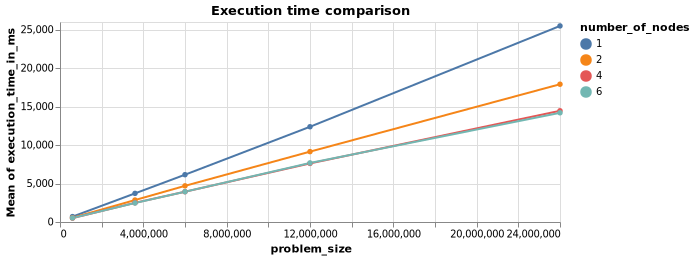
\includegraphics[width=.9\linewidth]{./images/exec_time.png}
\end{center}

Speedup comparison
\begin{center}
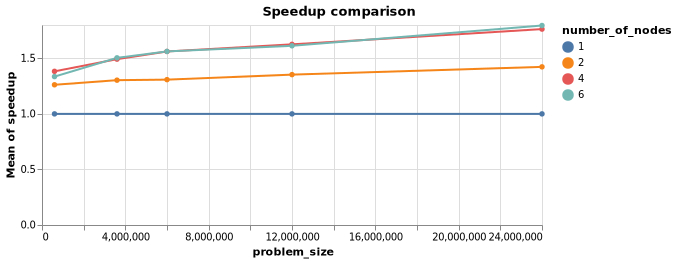
\includegraphics[width=.9\linewidth]{./images/speedup.png}
\end{center}

As you can see from these charts that as size increases the
distributed implementation is faster. But the speedup is not linear.
As number of nodes increases upto 6, the speedup achieved is only 1.5.

\begin{enumerate}
\item Runtime analysis
\label{sec:orgc32b61b}
\begin{itemize}
\item Number of iterations for the distributed data removal is equal to
the number of nodes
\item In each iteration, we pass through the entire list O(N). Since we do
this for M iterations, total number of times the list gets examined
is O(M x N)
\item In each iteration m, we also copy O(N/M) elements from one node to all
(m, M) nodes
\begin{itemize}
\item In the first iteration, there is a many to one copy of O(N/M)
elements from node 1 to all (m-1) nodes
\item In the second iteration, there is a many to one copy of O(N/M)
from node 2 to all (m > 2) nodes
\item In each iteration the number of nodes involved in the many-to-one
copy transfer shrinks. (Starting from m-1 nodes in the first
iteration to 0 in the last iteration)
\end{itemize}
\item In each iterations, node m contains the unique list of elements.
This can be saved in parallel at the end using a distributed file
system or the elements can be copied to node 1 and saved (as is
common to do so, in HPC systems)
\end{itemize}
\end{enumerate}

\subsubsection{Processing millions of specialties in parallel}
\label{sec:org7fa5240}
\begin{itemize}
\item The millions of specialties and their corresponding ids can be
hosted in parallel.
\item Since the (id, specialty) pair can be assumed to be unique, we can
use a simple routing function to route any (id, specialty) pair
to a node m (in a cluster of M nodes)
\item Example distribution function: node\textsubscript{id} = modulo(id, M)
\item Example (id, specialty) pairs
\end{itemize}
\begin{verbatim}
[
(7231, "algorithms"), 
(2134, "security"), 
(4532, "compilers"),
(3000, "journalism")
]
\end{verbatim}
\begin{itemize}
\item After applying the routing function, node\textsubscript{id} = module(id, M).
Assuming M = 3
\end{itemize}
\begin{center}
\begin{tabular}{lll}
Node0 & Node1 & Node2\\
\hline
(3000, "journalism") & (7231, "algorithms") & (4532, "compilers")\\
 & (2134, "security") & \\
\end{tabular}
\end{center}
\begin{itemize}
\item Now the same routing function can be applied on the list of IDs
before lookup and routed to the appropriate node for the specialties lookup
\item Each node m, can also use a separate hashmap on the id facilitating
faster specialty lookup
\end{itemize}

\begin{enumerate}
\item Runtime analysis
\label{sec:org1682d50}
\begin{itemize}
\item The (id, specialty) pair can be processed in parallel in M nodes
during the table construction in memory.
\begin{itemize}
\item Runtime: O(N/M)
\end{itemize}
\item Communication between nodes is dependent on the skewness of the
data. If there are lot more ids that end with 1 after applying the
routing function, then node 1 will get a lot of (id,specialty) pairs
to host
\item This design works well only when the data/routing function balances
the data equally among M nodes
\end{itemize}
\end{enumerate}

\subsubsection{Millions of (id, specialty) pairs and millions of ids}
\label{sec:org5c22628}
\begin{itemize}
\item We can use the design above to host millions of (id, specialty)
pairs in M nodes
\item We can use the "distributed duplicate removal" design above to
filter ids of duplicates. This retains the order of inputs ids while
removing duplicates
\item Example specialties table
\end{itemize}
\begin{center}
\begin{tabular}{lll}
Node0 & Node1 & Node2\\
\hline
(3000, "journalism") & (7231, "algorithms") & (4532, "compilers")\\
 & (2134, "security") & \\
\end{tabular}
\end{center}
\begin{itemize}
\item Example unique ids in memory. Note that the routing function hasn't
been applied to the ids yet. So, the ids in node m may not find the
specialties in node m and may have to communicate with another node
to find it's specialty
\end{itemize}
\begin{center}
\begin{tabular}{rrr}
Node0 & Node1 & Node2\\
\hline
7231 & 2134 & 3000\\
4532 &  & \\
\end{tabular}
\end{center}
\begin{itemize}
\item For each iteration m in range(0, M)
\begin{itemize}
\item node m - acts as the sender
\item all nodes in range (m, M) nodes act as the receiver
\item Get all ids in node m, and apply the routing function. Send
lookup request to the corresponding node. Receive specialty name
from the 
\begin{itemize}
\item Example: In node 0
\item routing\textsubscript{fn}(7231) -> node1 -> lookup\textsubscript{specialty}(incoming\textsubscript{id}) ->
return\textsubscript{result}\textsubscript{from}\textsubscript{node1}\textsubscript{to}\textsubscript{node0}
\end{itemize}
\end{itemize}
\item After M iterations, the specialties in M nodes look as below
\end{itemize}
\begin{center}
\begin{tabular}{lll}
Node0 & Node1 & Node2\\
\hline
algorithms & security & journalism\\
compilers &  & \\
\end{tabular}
\end{center}
\begin{itemize}
\item These results can be printed in order by traversing nodes 0 to M-1
\end{itemize}

\subsection{Unit tests}
\label{sec:orge0bddaf}
\begin{itemize}
\item Unit tests are in file test/check.f90. You can run them with `make test`
\end{itemize}
\begin{verbatim}
arul@arul-Serval ~/d/ornl-assignment (main)> fpm test
ornl-assignment.f90                    done.
parallel-work.f90                      done.
check.f90                              done.
libornl-assignment.a                   done.
main.f90                               done.
ornl-assignment                        done.
check                                  done.
[100%] Project compiled successfully.
# Testing: extract_digits_suite
  Starting random_string(length=0) ... (1/4)
       ... random_string(length=0) [PASSED]
  Starting random_string(length=5) ... (2/4)
       ... random_string(length=5) [PASSED]
  Starting random_string(length=50) ... (3/4)
       ... random_string(length=50) [PASSED]
  Starting random_string(length=500) ... (4/4)
       ... random_string(length=500) [PASSED]
# Testing: remove_duplicates_suite
  Starting rm_duplicate_string(list_size=2) ... (1/3)
       ... rm_duplicate_string(list_size=2) [PASSED]
  Starting rm_duplicate_string(list_size=10) ... (2/3)
       ... rm_duplicate_string(list_size=10) [PASSED]
  Starting rm_duplicate_string(list_size=100) ... (3/3)
       ... rm_duplicate_string(list_size=100) [PASSED]
# Testing: specialties_lookup
  Starting ids_string_to_int ... (1/7)
       ... ids_string_to_int [PASSED]
  Starting specialties_lookup(table_size=1, ids_list=10) ... (2/7)
       ... specialties_lookup(table_size=1, ids_list=10) [PASSED]
  Starting specialties_lookup(table_size=10, ids_list=10) ... (3/7)
       ... specialties_lookup(table_size=10, ids_list=10) [PASSED]
  Starting specialties_lookup(table_size=100, ids_list=10) ... (4/7)
       ... specialties_lookup(table_size=100, ids_list=10) [PASSED]
  Starting specialties_lookup(table_size=1, ids_list=1) ... (5/7)
       ... specialties_lookup(table_size=1, ids_list=1) [PASSED]
  Starting specialties_lookup(table_size=1, ids_list=0) ... (6/7)
       ... specialties_lookup(table_size=1, ids_list=0) [PASSED]
  Starting specialties_lookup(table_size=1, ids_list=100) ... (7/7)
       ... specialties_lookup(table_size=1, ids_list=100) [PASSED]
\end{verbatim}
\end{document}
